\subsection{Persiapan \textit{kubernetes cluster}}

Tahapan ini merupakan tahapan persiaspan sebelum proses \textit{development}. Pada tahapan ini akan dibuat kubernetes \textit{cluster} pada komputer lokal dengan kakas \textit{kind}. \textit{Cluster} yang dibuat akan memiliki 4 nodes dengan spesifikasi 1 \textit{master node} dan 3 \textit{worker node}. Digunakan \textit{command} \textbf{kind create cluster --config cluster.yaml} dengan file konfigurasi yang dapat dilihat dibawah ini.

\begin{figure}[h]
  \centering
  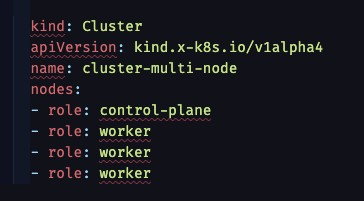
\includegraphics[width=1\textwidth]{resources/appendix/pembuatan-cluster.jpg}
  \caption{konfigurasi pembuatan \textit{cluster} dengan kakas \textit{kind}}
  \label{fig:konfigurasi-pembuatan-cluster}
\end{figure}

\begin{figure}[h]
  \centering
  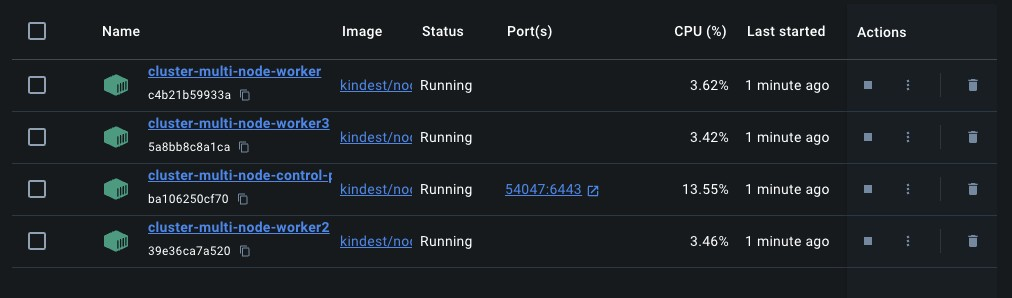
\includegraphics[width=1\textwidth]{resources/chapter-4/cluster-kind.jpg}
  \caption{Hasil \textit{cluster} dengan kakas \textit{kind}}
  \label{fig:hasil-cluster-kind}
\end{figure}

\pagebreak